\documentclass[]{article}
\usepackage[backend=biber, style=numeric]{biblatex}
\usepackage{paralist}
\usepackage{hyperref}
\usepackage{float}
\usepackage{graphicx}
\usepackage{booktabs}
\graphicspath{ {./images/} }

\addbibresource{researchProposal.bib}
\newtheorem{researchquestion}{RQ}

%opening
\title{Research Proposal \\
	A YOLOv8-based Analysis of Image Augmentation Techniques for Vehicle Detection in Adverse Weather Conditions}
	\author{
		Alexander Van Hecke \small(852631385) \and 
		Frederik Lefever    \small(838836963)}

\begin{document}

\maketitle

\begin{abstract}
	Vehicle detection is an important aspect of semi-automated traffic monitoring and surveillance.  We propose to investigate whether the technique of image augmentation can be used to increase the accuracy of vehicle detection in adverse weather conditions.  The study will evaluate whether the use of image augmentation to train a YOLO\small{v8} model increases accuracy compared to a baseline model.  We also propose to compare the effect of training with augmentated images to that of training with actual images of traffic in adverse weather conditions. To this extent we will train a YOLO\small{v8} model with actual images and compare with the same baseline model and the accuracy obtained from the first model. Our main hypothesis is that image augmentation can indeed be used to improve the accuracy of vehicle detection in adverse weather conditions. Our secondary hypothesis is that the accuracy of a model derived from augmented images falls within statistically insignificant margins when compared to a model obtained from actual images.  
\end{abstract}

\section{Introduction}

	Adverse weather conditions such as rainfall, snow and fog are widely considered to have an effect on traffic flow. Traffic breakdown occurs when demand exceeds capacity in some part of a transportation network and in \cite{stralenInfluenceAdverseWeather2015} it is shown that the odds of traffic breakdown at bottleneck locations are significantly increased by rainfall.  This can lead to considerable economic damage and provides a strong incentive to mitigate this problem as much as possible.
	
	Traffic monitoring and dynamic flow controle can be part of a mitigation strategy. The current technology behind traffic monitoring largely uses vehicle detection in images captured from CCTV cameras positioned next to highways. However, vehicle detection in images can be influenced by adverse weather conditions.
	
	We propose to investigate the effect of image augmentation on the robustness of YOLO{\small v8}-based vehicle detection models. In particular, we propose to investigate the effect of artificially adding rain, fog and snow to real clear weather images of highways. Compared to the standard YOLO{\small v8} model, we expect to see an improvement of the Mean Average Precision (mAP) for vehicle detection in models derived from YOLO{\small v8} by training on the augmented images. We chose YOLO{\small v8} as our base model because of its modernity and popularity. Also, YOLO{\small v8} is well-documented, both as a ready-to-use product and in scientific literature. Finally, YOLO{\small v8} is an open-source software, licensed under AGPL-3.0. All artifacts produced by the proposed study will hence be made available through a public GitHub repository.  
	
	The immediate relevance of our findings can be explained in terms of the above mentioned applications to traffic monitoring. But it is possible that some results could be of value in other weather-sensitive applications, such as surveillance of skiers on mountain slopes.

\section{Literature review}

	In the context of machine learning, image augmentation can broadly be defined as the automated creation of variation in actual image datasets. This technique can be used to avoid a learning algorithm overfitting the data. Overfitting occurs when a learning algorithm learns a function in such a way that it perfectly models the training data, but is unable to generalize beyond the training data. Large volumes of data with sufficient variation can alleviate the problem of overfitting. Yet sometimes sampling data from an application domain is nontrivial, eg. when learning from medical images.  Image augmentation can be used to artificially create additional images, or to add some sort of noise to images in order to make the resulting model more robust.
	
	A comprehensive survey of modern image augmentation techniques is presented in \cite{shortenSurveyImageData2019}. Several approaches such as geometric transformations, color space augmentations, kernel filters, mixing images, random erasing, feature space augmentation, adversarial training, generative adversarial networks, neural style transfer, and meta-learning, are explained. \cite{xuComprehensiveSurveyImage2023} offers a more recent survey of image augmentation techniques as used in deep learning. This survey introduces a novel taxonomy, where image augmentation algorithms are classified as either model-free, model-based, or optimizing policy-based. The objectives of image augmentation are explained by analyzing the challenges encountered when deploying deep learning models for computer vision. A theoretical framework for understanding data augmentation is described in \cite{daoKernelTheoryModern2019}. First a general model of augmentation as a Markov process is given, and it is shown that kernels appear naturally with respect to this model. Next, a more direct analysis of the effect of augmentation on kernel classifiers is offered.
	
	The effectiveness of image augmentation on the classification of images with deep learning is discussed in \cite{perezEffectivenessDataAugmentation2017}. Simple techniques, such as cropping, rotating, and flipping images are compared. Additionally this paper reports on experiments with generative adversarial neural networks to learn augmentation strategies.
	
	Research similar to the proposed research can be found in \cite{kumarObjectDetectionAdverse2023}. The central question in \cite{kumarObjectDetectionAdverse2023} is whether YOLO{\small v8} can be improved through transfer learning to detect objects in adverse weather. This paper supports the hypothesis that training with actual images of adverse weather conditions significantly improves the detection performance compared to the standard YOLO{\small v8} model. An enhanced YOLO\small{v8}-based model for vehicle detection in foggy weather conditions is the focus of \cite{liVehicleDetectionFoggy2022}. The approach used to create the enhanced model is interesting in that the trainingset is obtained from 350 traffic images that are augmented with a fog-effect and subsequently dehazed with the multi-scale retinex with color restoration (MSRCR) algorithm. The final trainingset is then composed of the original images, fogged images and dehazed images. Whereas results in \cite{liVehicleDetectionFoggy2022} are reported with autonomous vehicles in mind, \cite{songVisionbasedVehicleDetection2019} specifically targets vehicle detection and counting in highway management.  A new segmentation method is proposed to divide a depicted highway road surface into a distal and a proximal area. Using this separation a YOLO{\small v3} model is trained to detect the type and location of vehicles. To estimate vehicle count and trajectories the Oriented FAST and Rotated BRIEF (ORB) algorithm is added to the image processing pipeline.
	

\section{Research questions}

	The image augmentation techniques described in the literature are numerous and varied, ranging from simple geometric transformations to the addition of noise and the changing of color, saturation and hue parameters. We propose to investigate the effect of \textit{thematic} image augmentation consisting in the addition of rain, fog and snow to clear weather images. At the more general level, we aim to answer following questions:

	\begin{researchquestion}
		\label{rq1}
		Given that the standard YOLO{\small v8} model is used as a comparative baseline and trained with thematically augmented images, will the resulting model then be more accurate as measured by the mean average precision (mAp) at 0.50-0.95 IoU, in predicting the location of vehicles in actual images of traffic in adverse weather conditions?
	\end{researchquestion}

	Furthermore, to appreciate the value of image augmentation in contexts where data is not necessarily scarce, we pose two additional questions:
	\begin{researchquestion}
		\label{rq2}
		Given that the standard YOLO{\small v8} model is used as a comparative baseline and trained with actual images of traffic in adverse weather conditions, will the resulting model then be more accurate as measured by the mean average precision (mAP) at 0.50-0.95 IoU, in predicting the location of vehicles in actual images of traffic in adverse weather conditions?
	\end{researchquestion}

	\begin{researchquestion}
		\label{rq3}
		Given a model obtained by training the standard YOLO{\small v8} model with thematically augmented images of traffic in adverse weather conditions, and a model obtained by training the standard YOLO{\small v8} model with actual images of traffic in adverse weather conditions, will both models then predict the location of vehicles in actual images of traffic in adverse weather condition with similar accuracy as measured by their respective mean average precision (mAP) at 0.50-0.95 IoU?
	\end{researchquestion}

\section{Research method}
\subsection{Measuring model accuracy}

	To estimate the robustness of vehicle detection models, we use the mean average precision (mAP) at 0.50-0.95 IoU, henceforth simply referred to as ``mAP''. The mAP is an aggregate metric based on the confusion matrix, the intersection over union (IoU), recall and precision. In this study, we only consider two relevant classes of vehicles, namely ``car'' and ``bus''.

\subsubsection{Calculation of the mAP at 0.50-0.95 IoU}

	The mAP is calculated by dividing the sum of the average precision ($AP$) per class by the number of classes $N$.  In our study $N = 2$ (``car'' and ``bus'').
	
	\[
	mAP = \frac{1}{N} \sum_{i=1}^{N} AP_i
	\]

	In summary, the $AP$ of a model is obtained by following steps:

	\begin{center}
		\begin{compactenum}
			\item Use model to generate prediction scores
			\item Map prediction scores onto class labels
			\item Construct the confusion matrix
			\item Calculate precision and recall for a set of IoU thresholds (0.50-0.95)
			\item Calculate area under precision-recall curve
			\item Calculate average precision
		\end{compactenum}
	\end{center}

	The IoU metric is used to evaluate the performance of object detection by quantifying the fit between the ground truth bounding box and the predicted bounding box.
	
	\begin{figure}[h]
		\centering
		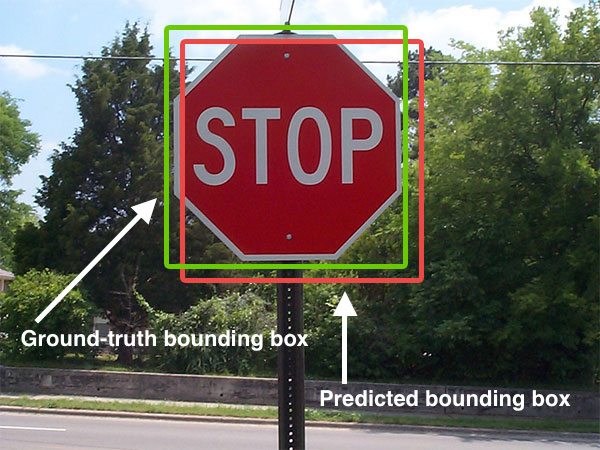
\includegraphics[width=5cm]{Intersection_over_Union_-_object_detection_bounding_boxes.jpg}
		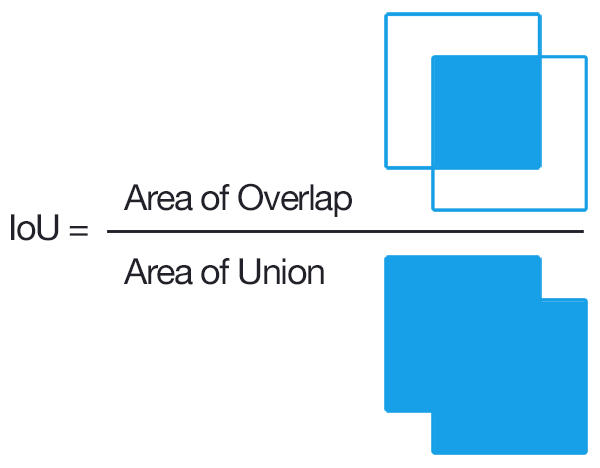
\includegraphics[width=5cm]{Intersection_over_Union_-_visual_equation.png}
		\caption{Images from Wikipedia \footnotesize{(\url{https://en.wikipedia.org/wiki/Jaccard_index})}}
	\end{figure}
	
	By using a lower bound for the value of the IoU metric, one can discriminate between positive and negative predictions. The IoU metric can then be used to calculate recall and precision. In the context of traffic management, it seems reasonable to slightly favour recall over precision and choose an IoU threshold to reflect this preference. However, choosing a good IoU threshold is itself an optimization process. For comparing models, optimizing the IoU threshold is unnecessary. Instead, we calculate AP as an average of AP's calculated for a set of IoU thresholds per class.

\subsection{Data collection}

	Two open-source datasets are used for this research. The DAWN dataset \cite{bw1x-yh39-20} is a collection of 1000 images from real-traffic environments in adverse weather conditions. The images are divided into four sets of weather conditions: fog, snow, rain and sandstorms. They are labelled according to the categories relevant for current research (``car'' and ``bus'') and annotated with object bounding boxes. We use the DAWN dataset for both validation and training.
	
	The second dataset is the UA-DETRAC \cite{CVIU_UA-DETRAC} dataset. This dataset provides 140K traffic images taken at Beijing and Tianjin (China). Images of the UA-DETRAC dataset are divided into four weather categories: ``cloudy'', ``night'', ``sunny'' and ``rainy''. They are labelled ``car'', ``bus'', ``van'' and ``others''; and annotated with object bounding boxes. The dataset is split into a training dataset (DETRAC-Train-Images) and an evaluation dataset (DETRAC-Test-Images).   From the union of the train and test datasets, we only use images of the category ``sunny'' for data augmentation and training. No other images are used from the UA-DETRAC dataset. See Table \ref{table:datasets} for an overview.
	
	\begin{table}[H]
		\centering
		\begin{tabular}{cccp{1.5in}}
			\toprule
			\textbf{dataset} & \textbf{labels} & \textbf{filter} & \textbf{number of images} \\
			\midrule
			\textbf{DAWN} & car, bus & fog, snow, rain &  \\
			\textbf{EU-DETRAC} & car, bus & sunny &  \\
			\bottomrule
		\end{tabular}
		\caption{Datasets used}
		\label{table:datasets}
	\end{table}

\subsection{Model selection}
 
	For vehicle detection we chose an open source convolutional neural network called YOLO{\small v8} \cite{yolov8_ultralytics}. We use this model in transfer learning and as a reference for derived models. YOLO{\small v8} is trained on the Microsoft COCO dataset \cite{linMicrosoftCOCOCommon2015a} and capable of detecting object categories ``car'' and ``bus''.

\subsection{Experiments}

	The chosen augmentation software imgaug \cite{imgaug} (version 0.4.0) cannot add sandstorm effects to images, so we start by creating a subset of the DAWN dataset by excluding all images of the weather category ``sandstorm''. The resulting subset is then randomly partitioned with a 80/20 ratio. The larger part is denoted by DAWN-train and the smaller part by DAWN-test.

	Next we establish a baseline measurement, by presenting the DAWN-test set to the standard YOLO{\small v8} model and determine its mAP over the ``car'' and ``bus'' classes. Then, we compose the union of the DETRAC-Train-Images and DETRAC-Test-Images and from it extract images of the weather category ``sunny''. The extracted images are used to produce three distinct trainingsets by augmenting them with fog, rain and snow using imgaug \cite{imgaug}. The obtained trainingsets are denoted resp. DETRAC-fog, DETRAC-rain and DETRAC-snow. We then train the standard YOLO{\small v8} model with the union of the DETRAC-fog, DETRAC-rain and DETRAC-snow datasets. Finally, we determine the mAP of the new model over the  ``car'' and ``bus'' classes, by presenting it the DAWN-test set. Comparing the mAP of the baseline with the mAP of the new model should provide some ground for answering the first research question.

	To answer the second research question, we train the standard YOLO{\small v8} model with the DAWN-train dataset and measure the mAP of the derived model. Like before, the mAP is calculated over the ``car'' and ``bus'' classes for the DAWN-test set.
	
	A schematic summary of the proposed research process is given in figure \ref{fig:experiment_process} and tables \ref{table:setuprq1} and \ref{table:setuprq2}.
	
	\begin{figure}[H]
		\centering
		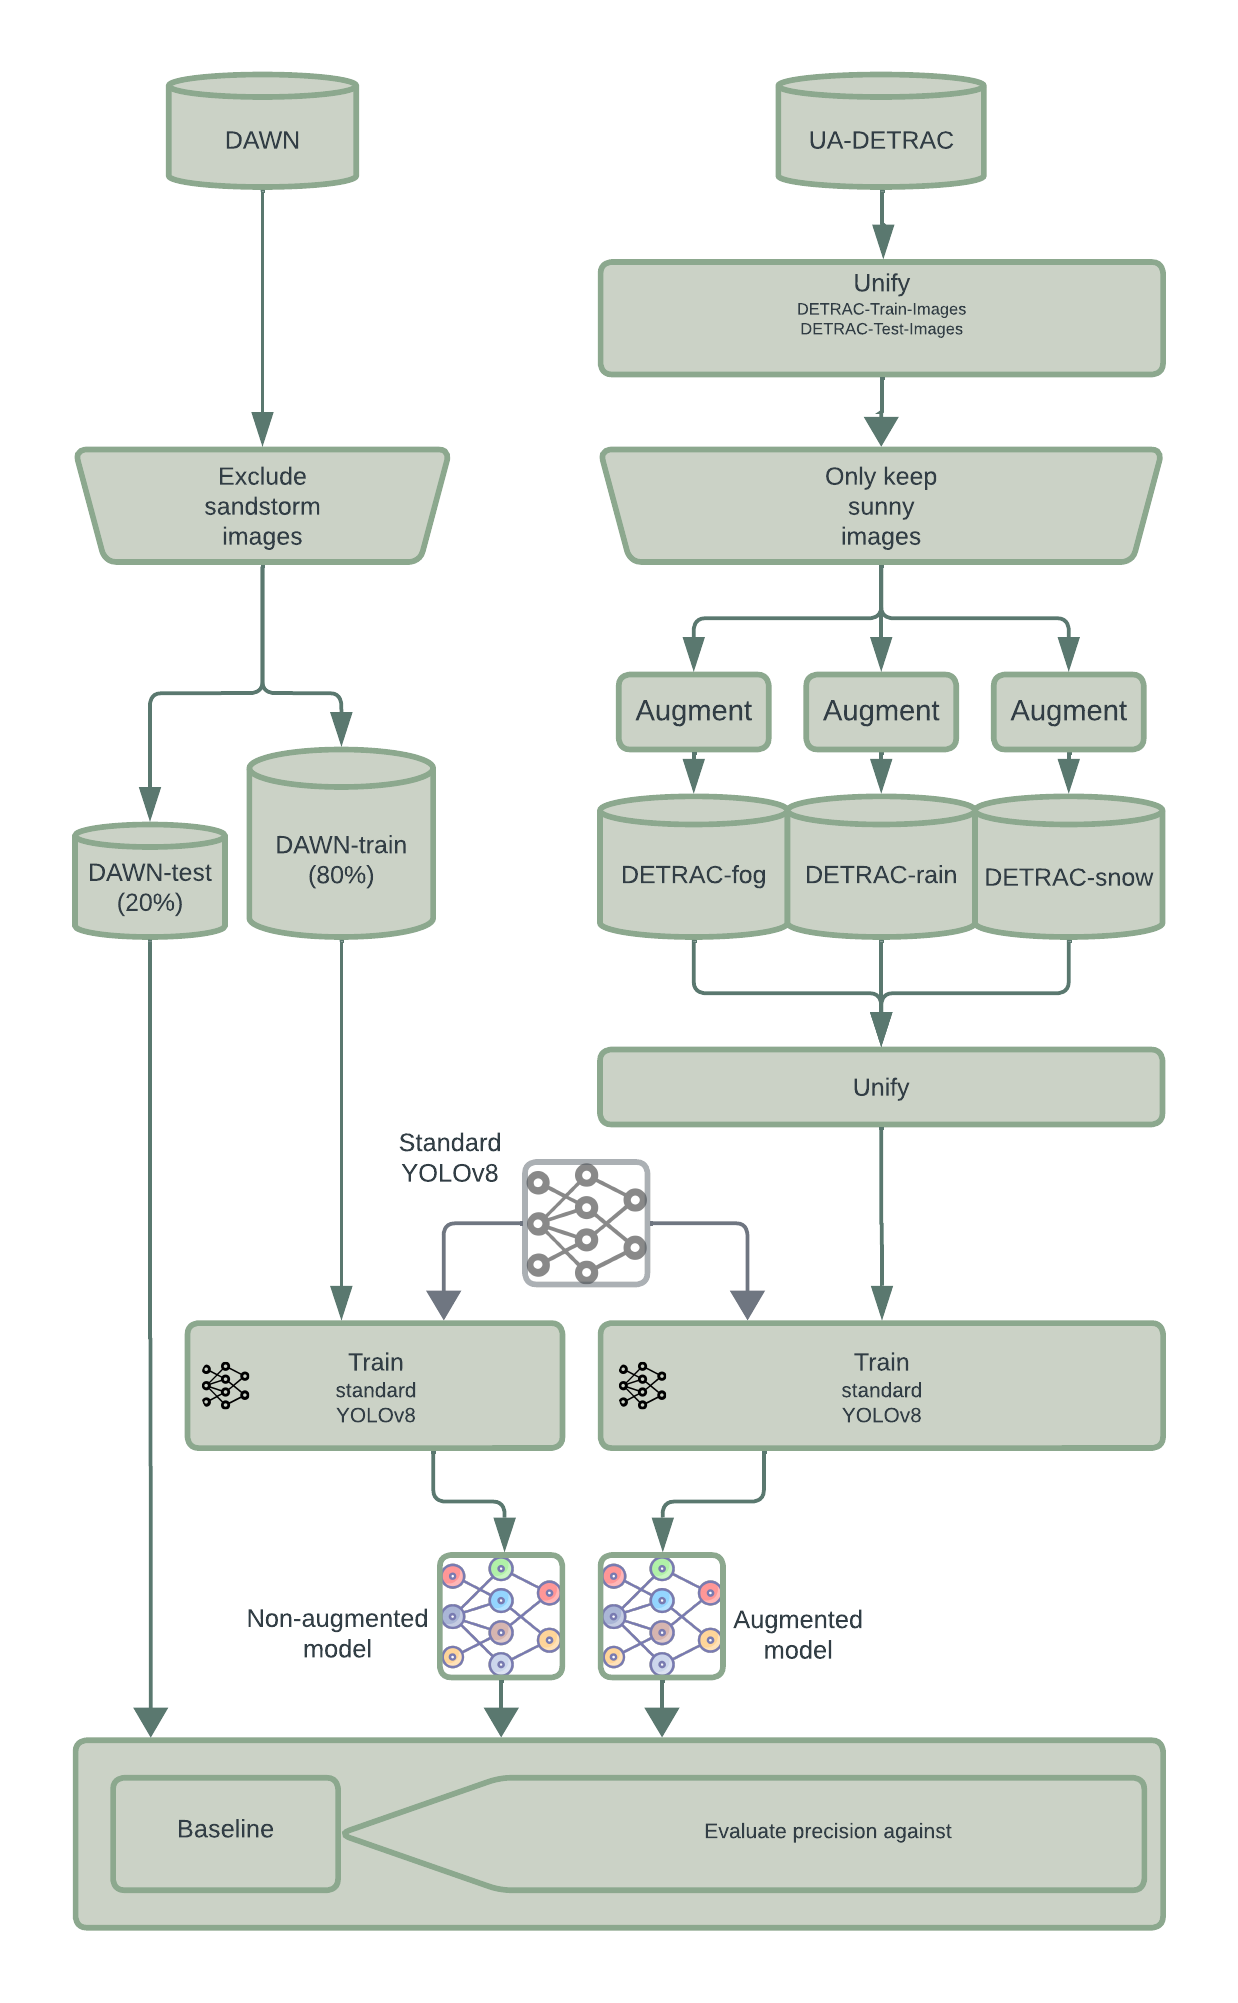
\includegraphics[scale=0.21]{Proposal_diagram.png}
		\caption{Schematic representation of proposed research}
		\label{fig:experiment_process}
	\end{figure}
	

	\begin{table}[H]
		\centering
		\begin{tabular}{lll}
			\toprule
			\textbf{measurement} & \textbf{training} & \textbf{data set} \\
			\midrule
			baseline & none & DAWN-test \\
			augmented images & DETRAC-train & DAWN-test \\
			\bottomrule
		\end{tabular}
		\caption{setup RQ \ref{rq1}}
		\label{table:setuprq1}
	\end{table}

	\begin{table}[H]
		\centering
		\begin{tabular}{lll}
			\toprule
			\textbf{measurement} & \textbf{training} & \textbf{data set} \\
			\midrule
			baseline & none & DAWN-test \\
			actual images & DAWN-train & DAWN-test \\
			\bottomrule
		\end{tabular}
		\caption{setup RQ \ref{rq2}}
		\label{table:setuprq2}
	\end{table}

\section{Data analysis}

	Our approach to the proposed study will be that of a single case mechanism experiment. More specifically, we investigate the effect of differences in an independent variable $X$ being a model derived by transfer learning from YOLO{\small v8} on a dependent variable mAP. Since we only consider three models (standard YOLO{\small v8}, a model derived from augmented images and a model derived from actual images), the study does not produce a volume of data large enough to use statistical techniques.
	
	Our scientific hypothesis related to research question \ref{rq1} is that, for the detection of cars and busses in images of traffic in adverse weather conditions, the mAP at 0.50-0.95 IoU of a model obtained by transfer learning from the standard YOLO{\small v8} with thematically augmented images, is higher than the mAP at at 0.50-0.95 IoU of the standard YOLO{\small v8}. 	
	
	Related to research question \ref{rq2}, our scientific hypothesis is similar to the hypothesis related to research question \ref{rq1}. Ie, for the detection of cars and busses in images of traffic in adverse weather conditions, the mAP at 0.50-0.95 IoU of a model obtained by transfer learning from the standard YOLO{\small v8} with  \textit{actual} images, is higher than the mAP at 0.50-0.95 IoU of the standard YOLO{\small v8}.  
	
	The statistical significans of the observed differences in accuracy must be left undecided in this study. Yet we will attempt to give an explanation of the causal relationship between image augmentation and improved accuracy of prediction.
	
	To conclusively answer research question \ref{rq3} in which we compare the accuracy of a model learned from augmented images with that of a model learned from actual images, our study provides insufficient evidence. Nevertheless, we will shortly present our intuitions based on our understanding of neural networks.
	

\section{Proposed time line}

The following tasks will have to be addressed (see Figure \ref{fig:timeline}) :
\begin{itemize}
	\item Dataset preparation
	\item Images augmentation
	\item Training models
	\item Evaluation of models
	\item Data analysis
	\item Write the report
\end{itemize}

\begin{figure}[H]
	\centering
	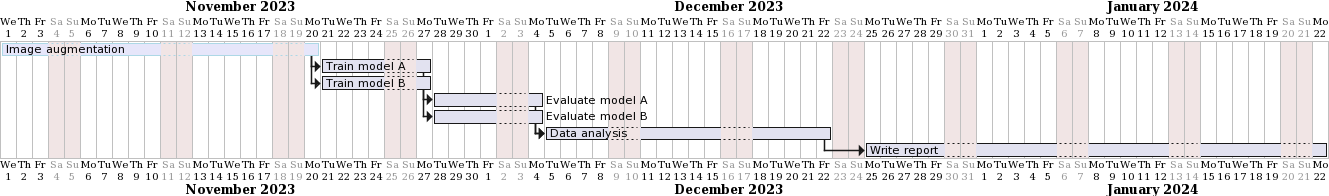
\includegraphics[width=\textwidth]{proposal-timing}
	\caption{Proposed timeline}
	\label{fig:timeline}
\end{figure}

\printbibliography

\end{document}
